\section{Industrial landscape, spin-offs and applications}
\label{sec:industry}

\subsection{Overview}
Commercial molten glass AM in 2026 consists of three small companies that build or operate molten-deposition machines (Evenline, Maple Glass Printing, Nobula3D), one that pioneered the field and went quiet (Micron3DP), one abandoned corporate patent filing (Corning), several indirect-route companies that compete for the same optics and microfluidics customers (Glassomer and the binder-jetting start-up Vitriform3D), and a small number of research-service arrangements (Mo-Sci with Northwestern, the RIT--Evenline partnership). No public company sells a molten glass printer; total disclosed external funding across the direct-route firms is below EUR~5 million. \Cref{tab:industry} gives the directory; the text below profiles each entity and then discusses application verticals and unit economics.

\begin{figure}[htbp]
  \centering
  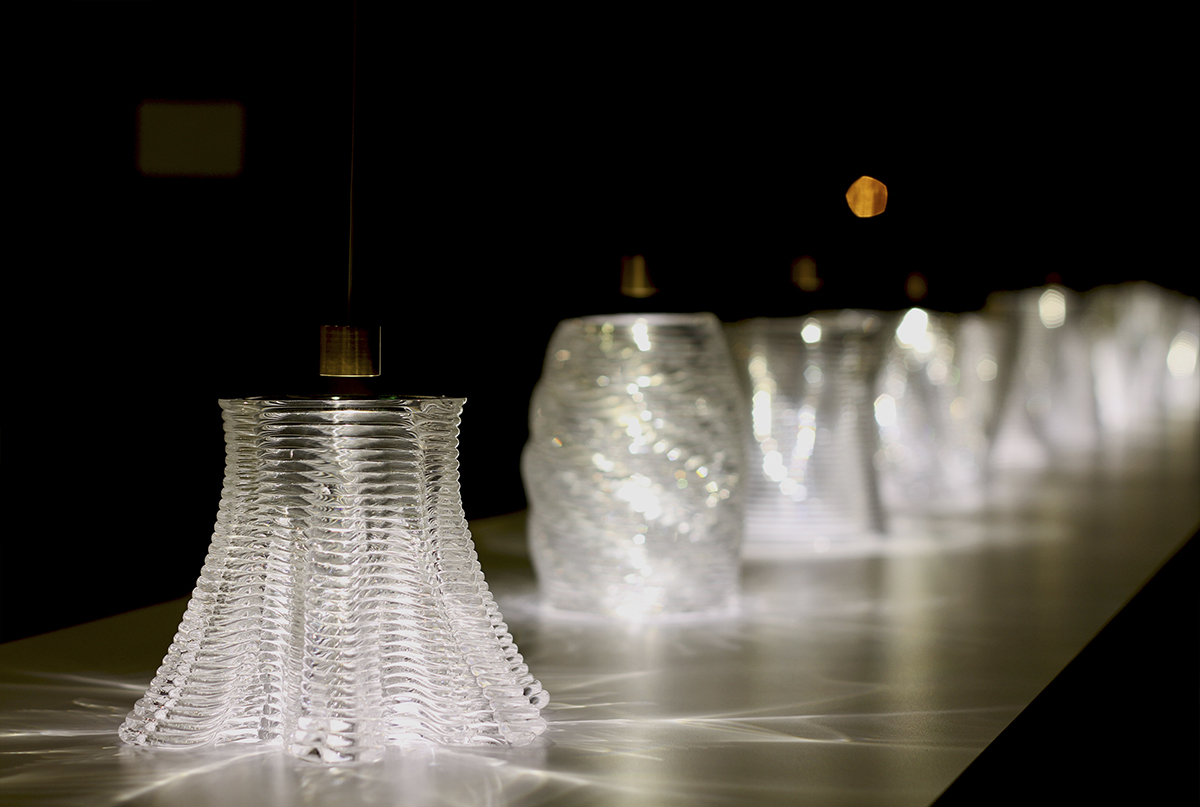
\includegraphics[width=0.8\linewidth]{commons_caustics.jpg}
  \caption{Printed soda-lime glass lamps from the MIT G3DP platform, illuminated from above; the periodic relief of the \SI{10}{mm} cords acts as an array of cylindrical lenslets and projects caustic patterns onto the table. The image illustrates both the optical signature of layer seams (\cref{sec:open}, Problem 2) and the lighting and art market that has been the first commercial outlet for molten glass AM. Photograph: Neri Oxman, Wikimedia Commons, CC BY-SA 4.0 \citep{commons_caustics}.}
  \label{fig:caustics}
\end{figure}

\subsection{Company profiles}
\paragraph{Evenline Inc.\ (Rochester, New York, USA).} Founded by Michael Stern, co-inventor of G3DP and G3DP2 at MIT and formerly of MIT Lincoln Laboratory, Evenline owns and operates the G3DP2 and the third-generation G3DP3 (``3D Glass Printer Mark III'') and sells printed art, lighting and design objects, custom parts for clients, and research services rather than machines \citep{evenline_web,acers2024recent,threednatives2025}. The G3DP3 prints \qtyproduct{325 x 325 x 380}{mm} from studio, container and float soda-lime glass at up to \SI{1200}{\celsius} with infrared thermographic calibration \citep{mit2024masonry,stern2024cgc}. The company hosted its printer at the Rochester Institute of Technology's College of Art and Design in 2023, where Stern teaches a digital-glass elective and where recycled bottle glass melted at \SI{2300}{\degree}F (\SI{1260}{\celsius}) is upcycled into printed objects; collaborations with NASA and DARPA on molten processing of lunar regolith are cited, and a Kickstarter campaign supported the recycled-glass programme \citep{rit2023}. With MIT it produced the interlocking masonry study \citep{mit2024masonry,mitnews2024bricks} and the recycled float and container glass study \citep{stern2024cgc}, and it stated that a next-generation G3DP4 could be a wide, low chamber for printing on large float sheets or a \SI{1700}{\celsius} machine for borosilicate, silica and regolith \citep{stern2024cgc}. Stern and Lizardo also founded Lios Design for printed architectural lighting. Intellectual property rests on the two MIT patents \citep{patent_us9919510,patent_us10464305,patent_us10266442}; funding is undisclosed.

\paragraph{Maple Glass Printing Pty Ltd (Melbourne, Australia).} Founded in 2017 by materials engineers Nick Birbilis and Darren Feenstra from Monash University; left university laboratories for its own premises in 2020, received a patent filing and commercialisation grant funding in late 2020 and a Canberra Innovation Network ICON grant, and introduced the Maple~2 and Maple~3 as its first commercial machines in 2022--2023 \citep{monash_maple,maple_ammedia,maple_aniwaa}. The Maple~3 (\qtyproduct{170 x 200 x 300}{mm}, cane feed, \SI{1000}{\celsius} nozzle, \SI{1.5}{mm} nozzle, \SI{0.1}{mm} minimum layer, approximately USD~45\,000) and the Maple~4 (2025, \qtyproduct{200 x 200 x 300}{mm}, \SI{100}{kg}, single-phase mains, one-click printing, automatic mesh levelling, magnetic bed) are sold to universities, studios and laboratories; the Vitri-Glass cane machine closes the loop from cullet \citep{maple_ammedia,threednatives2025,maple_web}. Applications cited are art and demonstration pieces, laboratory implements for neon and fibre-optic research, an architectural display project with Foster + Partners using recycled glass, and, in development, large-format robotic-arm printing for windows and fa\c{c}ades combined with wire-arc additive manufacturing \citep{maple_ammedia}. Process videos are on the company's YouTube channel, including a Formnext 2023 demonstration \citep{maple_youtube}. Birbilis co-authored the 2025 critical review \citep{critical2025}.

\paragraph{Nobula3D AB (Stockholm, Sweden).} A 2021 KTH spin-off from Michael Fokine's group, led by CEO Chunxin Liu, offering a complete system of desktop printer, fused-silica filament and software based on direct glass laser deposition (DGLD) \citep{nobula_kthventures,nobula_fabbaloo}. Specifications: non-contact CO$_2$-laser heating to \SI{2200}{\celsius}, \qtyproduct{180 x 180 x 100}{mm} build volume, \SI{0.1}{mm} Z resolution, \SIrange{100}{250}{\micro\metre} feature resolution, print speed up to \SI{200}{mm/s}, \qtyproduct{1000 x 400 x 600}{mm} footprint, \SI{50}{kg}, price on request \citep{nobula_aniwaa,threednatives2025}. Target applications are microlenses, microfluidics, lab-on-a-chip and organ-on-a-chip devices, fibre optics and art; the company markets ``precision hardware, software, computer vision and optical-grade glass'' \citep{nobula_web}. Backers include KTH Holding, the STING incubator and the European Innovation Council, with a EUR~2.5 million EIC Accelerator grant reported \citep{nobula_kthventures}.

\paragraph{Micron3DP Ltd (Kfar Saba / Hod Hasharon, Israel).} Founded by Eran Gal-Or, an extruder specialist, and the first company to show molten glass printing publicly in mid-2015 (soft glass at \SI{850}{\celsius}, borosilicate at a claimed \SI{1640}{\celsius}, \SI{100}{\micro\metre} layers, later a \qtyproduct{200 x 200 x 300}{mm} build volume) \citep{micron3dp_acers,micron3dp_3dprint2017}. Alpha units were installed in-house in 2017 and again reported in 2021 with plans for external beta testing; Gal-Or co-authored a glass-microfluidics paper with the University of Helsinki \citep{microfluidics2019}. No product release, funding round or activity after 2021 could be found; the company is listed as seeking a strategic investor. Its patent-pending extruder details were never published.

\paragraph{Corning Incorporated.} Corning's 2016 application for an induction-heated 80/20 platinum--rhodium barrel-and-nozzle crucible fed with glass rods, extruding beads onto a platform, is the only large-glass-company filing on molten extrusion AM in the corpus; it was published in 2021 and abandoned \citep{patent_corning2021}. Corning's contribution to the field is otherwise as the viscometry partner of the first G3DP paper \citep{klein2015} and as the supplier of the boro-aluminosilicate substrates that define one of the four viscosity curves in \cref{fig:vft}.

\paragraph{Glassomer GmbH (Freiburg, Germany).} Founded in April 2018 as a KIT spin-off by Bastian Rapp, Frederik Kotz and Dorothea Helmer, Glassomer sells silica-nanocomposite resins and granulates for SLA, FDM and injection moulding, and a printing service, converting parts to fused silica by debinding and sintering at about \SI{1300}{\celsius} \citep{glassomer_interview,kotz2017,mader2021}. Reported funding is about USD~0.8 million from EU programmes (EIC, Horizon 2020, ATTRACT) and prize money \citep{glassomer_crunchbase}. It is the reference competitor for the small-part optics and microfluidics market that Nobula targets with the direct route.

\paragraph{Vitriform3D (Knoxville, Tennessee, USA).} Founded by University of Tennessee students Alex Stiles and Dustin Gilmer, selected for the DOE Innovation Crossroads programme in 2022, and partnered with Oak Ridge National Laboratory's Manufacturing Demonstration Facility: robotic binder jetting of \SIrange{90}{95}{\percent} recycled glass powder with \SIrange{5}{10}{\percent} polymer binder, oven-set, for tiles, coasters, signs and, in development, building cladding \citep{ornl2026}. It is not a molten route but competes directly with Evenline and Maple in the recycled-glass architectural niche.

\paragraph{Research-service and development entities.} Mo-Sci LLC (Rolla, Missouri) is developing, with Northwestern University, a 3D printing method for soda-lime, borosilicate and sealing glasses for high-temperature components \citep{mosci_web}. MIT Lincoln Laboratory announced a \SI{250}{\celsius} direct-ink-writing route in 2022 \citep{acers2024recent}. The University of Utah's STELLAR project is an academic--industrial consortium rather than a company \citep{utah2025}.

\subsection{Application verticals}
\paragraph{Architecture and fa\c{c}ades.} This is the vertical in which molten deposition has a unique position because only the crucible-fed route reaches masonry scale. The Milan columns (2017) demonstrated free-standing structural glass at \SI{3}{m} with a design strength of \SI{4.1}{MPa} at a safety factor of ten \citep{inamura2018}; the 2024 masonry study demonstrated full-size interlocking units with ultimate strengths of \SIrange{64}{118}{MPa}, dimensional accuracy under \SI{1}{mm}, and a fully hollow design ready for implementation \citep{mit2024masonry}; and rib-on-plate printing directly onto \SIrange{3.2}{9.5}{mm} float glass, including coated products, showed a path to stiffened transparent panels \citep{stern2024cgc}. Structural qualification (Problem 6) and fire and impact performance remain open, as does the circular-economy claim, which is credible because the masonry units are adhesive-free and remeltable.

\paragraph{Custom optics and lenses.} Laser-filament printing produces fused-silica lenses, microlens arrays with \SI{0.12}{nm} roughness and cylindrical-convex elements \citep{kth2024microlens,luo2018quartz}, waveguides and free-standing fibre from SMF-28 \citep{hostetler2018sff}; the LGD homogeneity work targets optical, thermal and structural components \citep{lgd2024homog,grotesk2022}. For imaging-grade bulk optics the indirect routes currently lead on index homogeneity \citep{destino2018}, and the direct routes compete on speed and on the absence of shrinkage.

\paragraph{Hermetic microfluidics and chemical reactors.} Glass microfluidics printed by the indirect route have been used for on-line mass-spectrometric reaction monitoring \citep{microfluidics2019}, and L-PBF parts, although opaque, are proposed for continuous-flow reactors and structured catalysts where chemical inertness outweighs transparency \citep{datsiou2021}. Nobula and Glassomer both target lab-on-a-chip devices. Direct laser-filament printing of sealed channels remains a research topic; hollow tubes have been printed \citep{dgf2023tubes}.

\paragraph{Packaging and luxury goods.} Powder-fed DED of soda-lime onto bottles offers one-step decoration without moulds \citep{spirrett2023}; a 2026 review of packaging glasses situates such customisation within container-glass sustainability \citep{packaging2026}. Evenline's printed spiral vessels with designer Josh Owen and its commissioned awards are the luxury-object end of the same market \citep{threednatives2025}.

\paragraph{Nuclear waste vitrification and high-temperature vessels.} No molten glass AM work for vitrification was found; the relevance is indirect---the Fluegel viscosity model underlying process calibration was built partly on nuclear-waste glass data \citep{fluegel2007}, and the platinum--rhodium crucible technology of vitrification melters is what a high-temperature printer nozzle would borrow \citep{pgm2010}. Mo-Sci's sealing-glass development addresses high-temperature hermetic components \citep{mosci_web}.

\paragraph{Space and in-situ resource utilisation.} Molten lunar regolith simulant extruded from a platinum--rhodium crucible under vacuum, and laser-fused regolith glass-ceramics, are active research lines that reuse molten-glass printer architectures \citep{regolithreview2023,regolithvac2024}; Evenline cites NASA and DARPA collaborations \citep{rit2023}.

\paragraph{Art, lighting and design.} The first and still largest revenue stream: Evenline's studio production, Maple's artist customers, and Nobula's ``arts'' listing. The optical signature of layer seams (\cref{fig:caustics}) is an asset here.

\subsection{Unit economics and business cases}
The available data permit only order-of-magnitude statements, which are nevertheless informative.

\emph{Capital cost.} A cane-fed desktop machine is USD~45\,000 \citep{maple_aniwaa}; a laser-filament desktop machine is priced on request but built from a \SI{25}{W} CO$_2$ laser, a fibre feeder and a small motion stage \citep{kth2022bonding,nobula_aniwaa}; a crucible-fed architectural machine is a \SI{19}{kW} thermal module with custom cast-alumina crucible, three kilns, a four-axis CNC and an annealing lehr \citep{inamura2018}---a six-figure build that no vendor sells.

\emph{Operating cost.} Energy is \SI{15}{kW} at \SI{5.2}{kg/h} (about \SI{3}{kWh/kg}) for G3DP2 plus annealing, versus roughly \SI{1}{kWh/kg} for industrial container furnaces; the crucible and refractories are consumables on a weeks-to-months cycle \citep{inamura2018,mit2024masonry}. Cane-fed machines use hundreds of watts but at gram-per-minute rates, so the energy per kilogram is comparable or higher; the cane itself must be drawn from cullet at additional cost \citep{maple_ammedia}. Laser processes deposit millilitres per hour and are viable only for small, high-value parts.

\emph{Material yield.} Molten deposition is near-net-shape with no mould and no sprue; losses are the lead-in and lead-out layers (cut off and remelted) and the crucible heel. Evaporative loss in laser printing is within measurement error (\SI{-1.6 +- 2}{\percent}) \citep{kth2022bonding}. Compared with kiln casting into 3D-printed sand moulds, AM eliminates the disposable mould but adds hours of machine time per unit.

\emph{Batch viability.} The masonry study's argument is the general one for AM: printing wins where every unit differs (topology-optimised or site-specific fa\c{c}ade elements) or where the tooling for pressing and casting cannot be amortised, and it loses to pressed glass block for identical units in volume \citep{mit2024masonry}. With a G3DP3 cycle of roughly one hour per double-height unit plus annealing, a single machine yields of the order of \(10^{3}\) masonry units per year---sufficient for demonstration walls and bespoke fa\c{c}ades, not for building stock. The crossover batch size has not been published by any group and is identified as an open question (\cref{sec:open}, Problem 8).

\subsection{Industrial systems directory}
\begin{sidewaystable}[p]
  \centering\scriptsize
  \caption{Industrial systems directory: molten-deposition machines and the principal indirect-route competitors. Temperatures are the maximum glass-processing temperature stated by the company or in the cited literature.}
  \label{tab:industry}
  \begin{tabular}{@{}L{2.6cm}L{2.7cm}L{3.2cm}L{2.3cm}L{3.4cm}L{3.6cm}L{2.2cm}@{}}
    \toprule
    Company (location, founded) & Machine name & Material compatibility & Max extruder / process temp. & Target market & Commercial status (2026) & Refs.\\
    \midrule
    Evenline Inc.\ (Rochester NY, USA; MIT spin-off, M.\ Stern) & G3DP2; G3DP3 ``3D Glass Printer Mark III'' (\qtyproduct{325 x 325 x 380}{mm}) & Studio, container and float soda-lime glass, incl.\ recycled cullet; colour by frit & \SI{1200}{\celsius} extrusion; furnace to \SI{1260}{\celsius} & Art, lighting, design objects; architectural masonry and fa\c{c}ade prototypes; custom parts; research (NASA, DARPA, RIT) & Operating; sells parts and services, not machines; G3DP4 planned & \citep{evenline_web,mit2024masonry,stern2024cgc,rit2023}\\
    Maple Glass Printing (Melbourne, Australia; 2017, N.\ Birbilis, D.\ Feenstra) & Maple 2, Maple 3 (\qtyproduct{170 x 200 x 300}{mm}), Maple 4 (\qtyproduct{200 x 200 x 300}{mm}); Vitri-Glass cane machine & Soda-lime cane, incl.\ recycled; colours segregated & \(\approx\)\SI{1000}{\celsius} nozzle & Education, art studios, laboratories (neon, fibre optics), architecture demonstrators & Machines on sale (Maple 3 approx.\ USD 45\,000); Maple 4 launched 2025; large-format robotic system in development & \citep{maple_ammedia,maple_aniwaa,threednatives2025,monash_maple}\\
    Nobula3D AB (Stockholm, Sweden; 2021, KTH spin-off, CEO C.\ Liu) & Nobula glass 3D printer (DGLD; \qtyproduct{180 x 180 x 100}{mm}) & Fused-silica filament (Nobula filament); silica glass & \SI{2200}{\celsius} (CO\(_2\) laser, non-contact) & Micro-optics, microfluidics, lab-/organ-on-a-chip, fibre optics, art & Available on request; EIC Accelerator EUR 2.5 M; KTH Holding, STING & \citep{nobula_aniwaa,nobula_fabbaloo,nobula_kthventures,nobula_web}\\
    Micron3DP Ltd (Kfar Saba, Israel; 2015, E.\ Gal-Or) & Unnamed high-resolution glass printer (\qtyproduct{200 x 200 x 300}{mm}, \SI{100}{\micro\metre} layers) & Soda-lime; borosilicate (claimed) & \SI{850}{\celsius} soft glass; \SI{1640}{\celsius} borosilicate (claimed) & Microfluidics, healthcare, architecture, art & Alpha units 2017--2021; no product; seeking investor; no activity found after 2021 & \citep{micron3dp_acers,micron3dp_3dprint2017,microfluidics2019}\\
    Corning Incorporated (Corning NY, USA) & Patent application only: induction-heated Pt--Rh crucible/nozzle, rod feed & Silicate glasses as rods \(\ge\)\SI{1}{mm} & n.r.\ (Pt--Rh to \(\sim\)\SI{1600}{\celsius}) & Glass articles (generic) & Application published 2021, abandoned & \citep{patent_corning2021}\\
    \midrule
    Glassomer GmbH (Freiburg, Germany; 2018, KIT spin-off) & Materials for open SLA/FDM printers; printing and injection-moulding service & Fused silica (nanocomposite \(\to\) sinter) & Sintering \(\approx\)\SI{1300}{\celsius} (indirect) & Optics, microfluidics, medical, automotive & Operating; approx.\ USD 0.8 M grants and prizes & \citep{glassomer_interview,glassomer_crunchbase,kotz2017}\\
    Vitriform3D (Knoxville TN, USA; 2022 DOE Innovation Crossroads) & Robotic binder jetting of recycled glass powder & 90--95\% recycled glass + 5--10\% binder & Oven-set (indirect) & Tiles, coasters, signage; building cladding in development & Start-up with ORNL/MDF support & \citep{ornl2026}\\
    Mo-Sci LLC with Northwestern University (Rolla MO, USA) & Development programme & Soda-lime, borosilicate, sealing glasses & n.r. & High-temperature components, hermetic seals & R\&D & \citep{mosci_web}\\
    MIT Lincoln Laboratory (Lexington MA, USA) & Direct-ink-writing route, \(\le\)\SI{250}{\celsius} & Silicate solution + inorganic nanoparticles & \SI{250}{\celsius} (indirect) & Thermally stable structures & Research announcement 2022 & \citep{acers2024recent}\\
    \bottomrule
  \end{tabular}
\end{sidewaystable}
